
\begin{frame}{What is Document-level Machine Translation}
	\begin{figure}
	\centering
	\begin{minipage}{.4\textwidth}
		\centering
		\textbf{Sentence-level MT}\par\medskip
		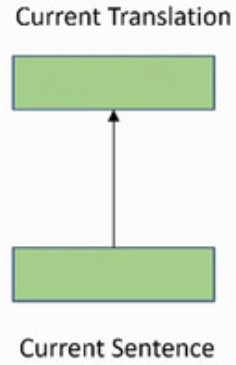
\includegraphics[width=.4\linewidth]{Images/dlmt}
	\end{minipage}%
	\begin{minipage}{.6\textwidth}
		\centering
		\textbf{Document-level MT}\par\medskip
		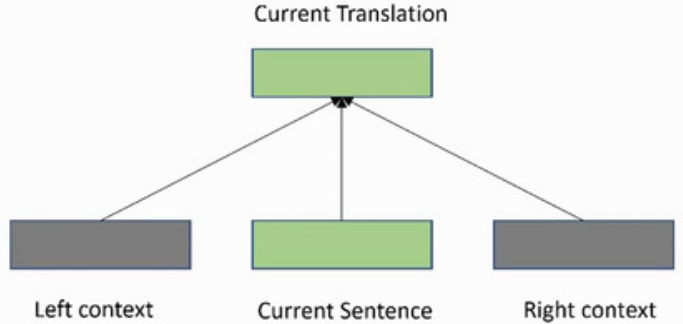
\includegraphics[width=.85\linewidth]{Images/slmt}
	\end{minipage}
	\end{figure}	
\end{frame}

\begin{frame}{Document-level MT $\leftrightarrow$ Context-aware MT}
	\begin{figure}
	\centering
	\begin{minipage}{.4\textwidth}
		\centering
		\textbf{Context-agnostic MT}\par\medskip
		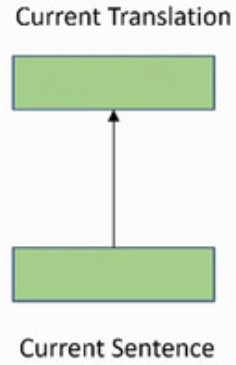
\includegraphics[width=.4\linewidth]{Images/dlmt}
	\end{minipage}%
	\begin{minipage}{.6\textwidth}
		\centering
		\textbf{Context-aware MT}\par\medskip
		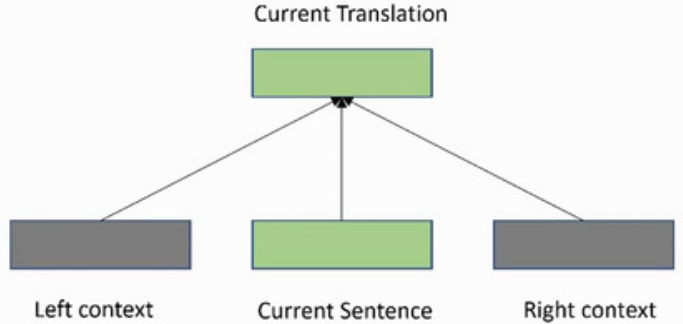
\includegraphics[width=.85\linewidth]{Images/slmt}
	\end{minipage}
	\end{figure}	
\end{frame}

\begin{frame}{Why Document-level NMT ?}
	
	\begin{itemize}
		\item<+(1)-|alert@+(1)>{Some recent results suggest that neural machine translation (NMT) "approaches the accuracy achieved by average bilingual  human  translators  [on  some  test  sets]” \cite{wu_googles_2016}
		}
		
		\item<+(1)-|alert@+(1)>{"In a pairwise ranking experiment, human raters assessing \textbf{adequacy} and \textbf{fluency} show a stronger preference for human over machine translation when evaluating documents as compared to isolated sentences." \cite{laubli_has_2018}
		}
	\end{itemize}
	
	
\end{frame}

\begin{frame}{Sentence-level NMT is inconsistent}
	\begin{center}
		\onslide<3->{%
			\begin{minipage}{0.75\textwidth}
				\RaggedRight
				\textbf{A}: Good Morning, \textcolor{blue}{Mr. President}.
			\end{minipage}
			\bigskip
		}
		\onslide<1->{%
			\begin{minipage}{0.75\textwidth}
				\RaggedRight
				\textbf{B}: How are \textcolor{blue}{you} today?
			\end{minipage}
			\bigskip
		}
		\onslide<2->{%
			\textbf{SENTENCE-LEVEL TRANSLATION}
			\medskip
			
			\begin{minipage}{0.75\textwidth}
				\RaggedRight
				\textbf{B}: Comment \textcolor{red}{vas-tu} aujourd'hui ?
	
			\end{minipage}
			\bigskip
		}
		\onslide<4->{%
			\textbf{DOCUMENT-LEVEL TRANSLATION}
			\medskip
			
			\begin{minipage}{0.75\textwidth}
				\RaggedRight
				\textbf{B}: Comment \textcolor{green}{allez-vous} aujourd'hui ?
			\end{minipage}
		}
	\end{center}
\end{frame}

\begin{frame}{How frequent are inconsistencies ?}
	\onslide<1->{%
		\cite{voita_when_2019} undertake a  human  study  on context agnostic translation :
			\begin{itemize}
				\item 2000 pairs of consecutive English sentences (S1 + S2) from OpenSubtitles2018
				\item translate to Russian with Transformer model \cite{vaswani_attention_2017}
			\end{itemize} 
	} 
	\onslide<2->{
	\begin{figure}
		\centering
		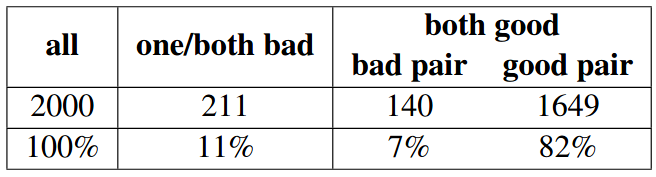
\includegraphics[width=0.7\linewidth]{Images/inconsistent_sentences}
		\label{fig:inconsistentsentences}
	\end{figure}
	}
	
\end{frame}

\begin{frame}{Which kind of inconsistencies?}
	\begin{figure}
		\centering
		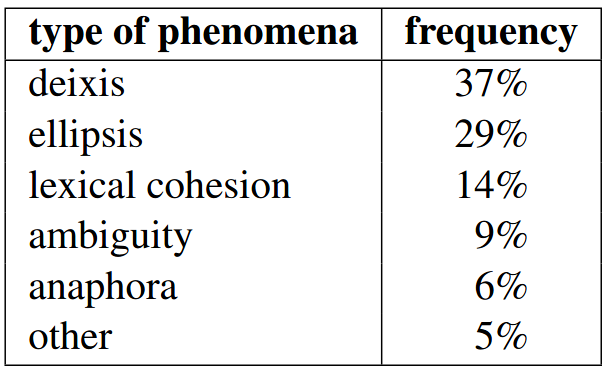
\includegraphics[width=0.7\linewidth]{Images/phenomena}
		\caption{Types of phenomena causing inconsistencies between English-Russian context-agnostic  translations  of  consecutive  sentences when placed in the context of each other.}
		\label{fig:phenomena}
	\end{figure}	
\end{frame}

\begin{frame}{Objectives}
	\begin{itemize}
		\item<+(1)-|alert@+(1)> \textbf{Design translation models and learning techniques} that solve inconsistencies by taking context into account;
		\item<+(1)-|alert@+(1)> \textbf{Evaluate such models} in a proper way;
	\end{itemize}
\end{frame}
